% !TeX root=../main.tex
\chapter{روش‌شناسی پژوهش و توسعه‌ی سامانه}
\label{ch:method}

\section{رویکرد پژوهش و مسیر توسعه}
\label{sec:method-research-process}

هدف این پژوهش، توسعه‌ی یک زنجیره‌ی یکپارچه برای مدل‌سازی، کنترل و پیاده‌سازی موتور صفحه‌ای با شناوری مغناطیسی (\lr{MLPM}) است. دستیابی مستقیم به یک سامانه‌ی فیزیکی پایدار، بدون در اختیار داشتن مدل قابل ارزیابی، محیط آزمون کنترل‌شده و رابط‌های مشخص میان کنترل‌کننده، حسگر و عملگر، با خطر آسیب به تجهیزات و دشواری جداسازی منشأ خطا همراه است. ازاین‌رو، روش پژوهش در دو مرحله‌ی پیوسته سازمان‌دهی شد. در مرحله‌ی نخست، سامانه‌ی معرفی‌شده در مرجع \cite{xuModularMaglevDesign2024d} به‌عنوان مبنای ساخت شبیه‌ساز انتخاب گردید و مدل دینامیکی، نگاشت جریان به پیچش، کنترل‌کننده، برنامه‌ریز مسیر و زیرساخت ارتباطی آن در یک حلقه‌ی بسته پیاده‌سازی شد. در مرحله‌ی دوم، معماری حاصل برای نمونه‌ی فیزیکی ساخته‌شده در این پژوهش به کار گرفته شد و اجزایی که به هندسه و سخت‌افزار واقعی وابسته بودند، بازطراحی شدند.

انتخاب یک سامانه‌ی مرجع در مرحله‌ی نخست به معنای یکسان فرض‌کردن آن با نمونه‌ی نهایی نیست. مدل مرجع امکان می‌داد پیش از تکمیل سخت‌افزار، نمایش شش‌درجه‌آزادی وضعیت، رابط پیچش مطلوب، ساختار کنترل فازی--\lr{PID}، تولید مسیر، اعمال قیود جریان، تبادل داده در \lr{ROS~2} و ثبت متغیرهای آزمایش توسعه یابند. پس از آماده‌شدن نمونه‌ی فیزیکی، همین رابط‌های مفهومی حفظ شدند؛ بااین‌حال، جرم متحرک، هندسه‌ی سیم‌پیچ و آرایه‌ی هالباخ، مدل مغناطیسی، تعداد کانال‌های فعال، حدود جریان، منبع بازخورد وضعیت و روش تخصیص جریان بر اساس سامانه‌ی ساخته‌شده تغییر کردند.

در مرحله‌ی شبیه‌سازی، \lr{Gazebo Harmonic} و موتور فیزیک \lr{DART} نقش فرایند را بر عهده دارند، \lr{MATLAB/Simulink} مرجع حرکت، کنترل و تخصیص جریان را محاسبه می‌کند و \lr{ROS~2 Jazzy} ارتباط میان این اجزا را برقرار می‌سازد. در مرحله‌ی فیزیکی، بازخورد شبیه‌ساز با اندازه‌گیری دوربین و نشانگرهای \lr{AprilTag} جایگزین می‌شود و جریان‌های تخصیص‌یافته، پس از عبور از رایانه‌ی رزبری‌پای، آردوینو و مدارهای قدرت، به سیم‌پیچ‌های واقعی اعمال می‌شوند. در نتیجه، مسیر کلی پژوهش از «مدل و شبیه‌ساز مرجع» به «نمونه‌ی فیزیکی و مدل ویژه‌ی آن» حرکت می‌کند، در حالی که ساختار سطح بالای کنترل و ارتباط میان دو مرحله مشترک باقی می‌ماند.

\begin{figure}[htbp]
	\centering
	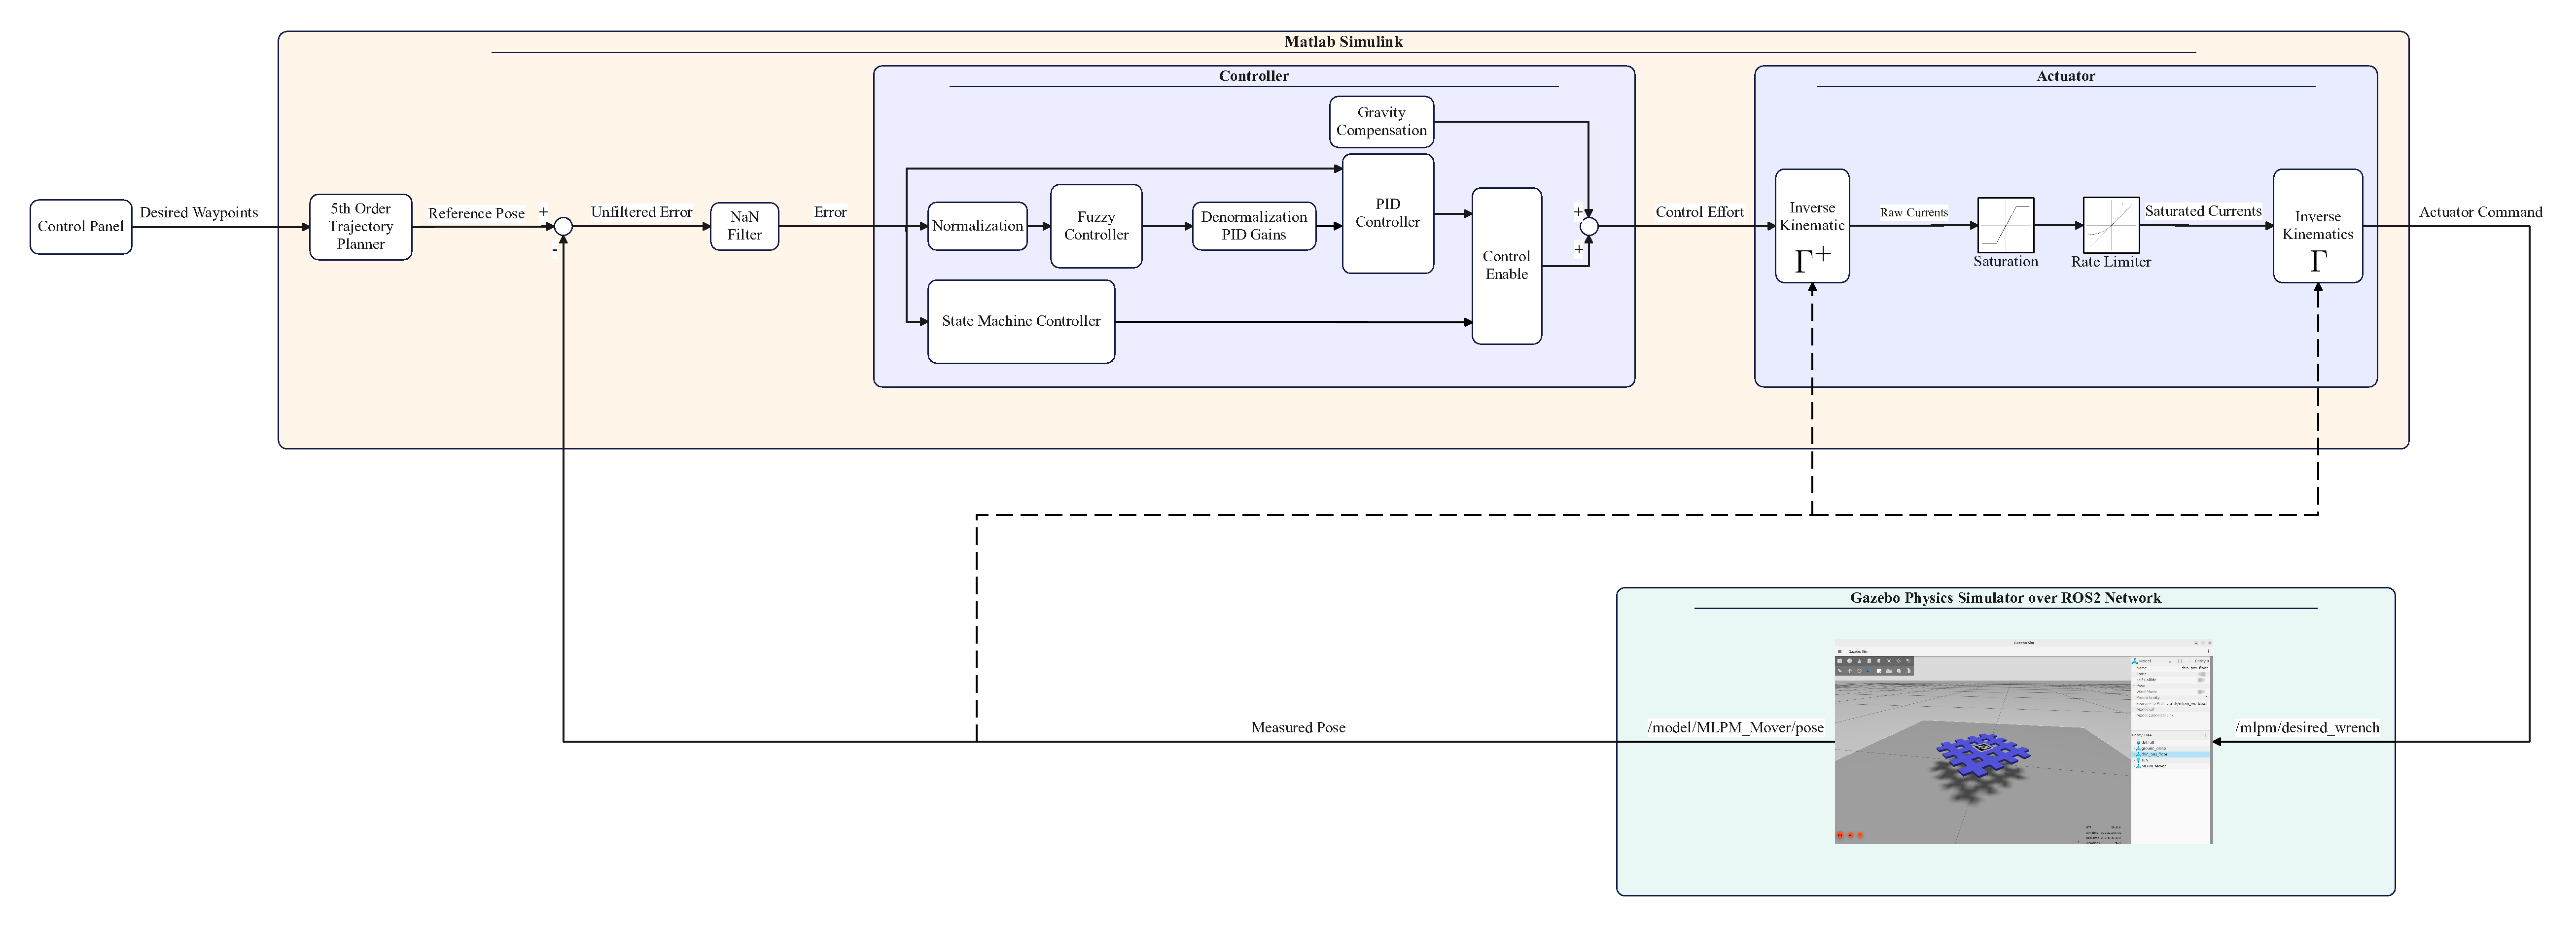
\includegraphics[width=0.95\textwidth]{img/system-overview.pdf}
	\caption{نمای کلی معماری شبیه‌سازی و حلقه‌ی کنترل در مرحله‌ی نخست}
	\label{fig:method-system-overview}
\end{figure}

بر این اساس، ابتدا مدل و محیط شبیه‌سازی مرجع تشریح می‌شود. سپس کنترل‌کننده و برنامه‌ریز مسیری که در هر دو مرحله به کار رفته‌اند ارائه می‌گردند. در ادامه، ساخت نمونه‌ی فیزیکی، مدل‌سازی مغناطیسی متناسب با هندسه‌ی آن، اندازه‌گیری وضعیت، تخصیص جریان هشت‌سیم‌پیچه، مدار راه‌انداز و رابط نظارتی توضیح داده می‌شوند. این ترتیب، علت ورود هر جزء به سامانه و نقشی را که در رسیدن از شبیه‌سازی به پیاده‌سازی واقعی ایفا کرده است روشن می‌سازد.

\section{مرحله‌ی نخست: مدل سامانه‌ی مرجع}
\label{sec:method-system-model}

\subsection{ساختار، مختصات و فرض‌های مدل}

سامانه‌ی مرجع از یک بخش متحرک حامل آرایه‌ی هالباخ و یک استاتور شامل شانزده سیم‌پیچ تشکیل شده است. هدف کنترلی، تعیین موقعیت و جهت‌گیری جسم متحرک در شش درجه آزادی است. بردار وضعیت هندسی و بردار پیچش به‌ترتیب به صورت

\begin{equation}
	\mathbf q=\begin{bmatrix}x&y&z&\alpha&\beta&\gamma\end{bmatrix}^{T},
	\qquad
	\mathbf W=\begin{bmatrix}F_x&F_y&F_z&T_x&T_y&T_z\end{bmatrix}^{T}
	\label{eq:method-pose-wrench}
\end{equation}

تعریف می‌شوند. زوایای $\alpha$، $\beta$ و $\gamma$ به‌ترتیب سمت‌گشت، تاب و غلت\LTRfootnote{Yaw: rotation about the vertical axis} را بیان می‌کنند. پارامترها و روابط الکترومغناطیسی این بخش از سامانه‌ی معرفی‌شده در \cite{xuModularMaglevDesign2024d} اخذ شده‌اند و مبنای مرحله‌ی شبیه‌سازی هستند.

\subsection{مدل دینامیکی بخش متحرک}
\label{subsec:method-mover-model}

در مدل اولیه، بخش متحرک یک جسم صلب در نظر گرفته شد. با صرف‌نظرکردن از مقاومت هوا و تلفات مکانیکی، معادلات انتقالی و دورانی آن در نزدیکی وضعیت‌های کاری مورد بررسی به صورت

\begin{align}
	m\ddot{x}&=F_x, & m\ddot{y}&=F_y, & m\ddot{z}&=F_z-mg,\label{eq:method-translational-eom}\\
	I_{xx}\ddot{\alpha}&=T_x, & I_{yy}\ddot{\beta}&=T_y, & I_{zz}\ddot{\gamma}&=T_z
	\label{eq:method-rotational-eom}
\end{align}

نوشته می‌شوند. اگر بردار حالت شامل موقعیت و سرعت هر شش درجه آزادی باشد، مدل حالت را می‌توان به صورت

\begin{equation}
	\dot{\mathbf x}_s=A\mathbf x_s+B\mathbf W+\mathbf g,
	\qquad
	\mathbf y=C\mathbf x_s+D\mathbf W
	\label{eq:method-state-dynamics}
\end{equation}

بیان کرد. ماتریس $A$ از شش بلوک انتگرال‌گیر مرتبه‌ی دوم تشکیل شده است، درایه‌های متناظر $B$ برابر $1/m$ برای حرکت انتقالی و $1/I_{jj}$ برای حرکت دورانی هستند، $C=I_{12}$ و $D=0_{12\times6}$ است. بردار $\mathbf g$ تنها در مؤلفه‌ی شتاب قائم مقدار $-g$ دارد. پارامترهای مدل مرجع در جدول \ref{tab:method-reference-dynamics} آمده‌اند.

\begin{table}[htbp]
	\centering
	\caption{پارامترهای دینامیکی بخش متحرک در شبیه‌سازی مرجع}
	\label{tab:method-reference-dynamics}
	\begin{tabular}{|c|c|}
		\hline
		جرم $m$ & $6.6\,\mathrm{kg}$\\ \hline
		$I_{xx}$ و $I_{yy}$ & $0.059\,\mathrm{kg\,m^2}$\\ \hline
		$I_{zz}$ & $0.12\,\mathrm{kg\,m^2}$\\ \hline
		شتاب گرانش $g$ & $9.81\,\mathrm{m/s^2}$\\ \hline
	\end{tabular}
\end{table}

\subsection{مدل تحلیلی جریان به پیچش}
\label{subsec:method-stator-model}

شانزده سیم‌پیچ مدل مرجع در آرایه‌ای $4\times4$ قرار دارند. اگر گام مکانی سیم‌پیچ‌ها $\tau$ باشد، مختصات مرکز آن‌ها از روابط

\begin{align}
	x_{c,j}&=(j-1)\tau-\frac{(n_c-1)\tau}{2},\quad j=1,\ldots,n_c,\label{eq:method-xcenter}\\
	y_{c,i}&=(i-1)\tau-\frac{(n_r-1)\tau}{2},\quad i=1,\ldots,n_r,\label{eq:method-ycenter}\\
	z_c&=0,\qquad n_r=n_c=4
	\label{eq:method-grid-params}
\end{align}

به دست می‌آیند. برای محاسبه‌ی اثر هر سیم‌پیچ، بردار فاصله‌ی مرکز آن تا متحرک به دستگاه مختصات متحرک تبدیل می‌شود:

\begin{equation}
	\mathbf c^{m}=R_z^{T}(\gamma)R_y^{T}(\beta)R_x^{T}(\alpha)
	\begin{bmatrix}x_c-x&y_c-y&z_c-z\end{bmatrix}^{T}.
	\label{eq:method-cm-vector}
\end{equation}

در مدل مرجع، مؤلفه‌های نیروی حاصل از واحد جریان سیم‌پیچ بر اساس روابط شناسایی‌شده‌ی \cite{xuModularMaglevDesign2024d} به صورت

\begin{align}
	F_x&=K_x\cos(\eta_x)\sin(\eta_y),\\
	F_y&=K_y\sin(\eta_x)\cos(\eta_y),\\
	F_z&=K_z\sin(\eta_x)\sin(\eta_y),
	\label{eq:method-force-components}
\end{align}

است که در آن

\begin{align}
	\eta_x&=\frac{\pi}{\tau}c_1^m,\qquad \eta_y=\frac{\pi}{\tau}c_2^m,\label{eq:method-eta}\\
	K_x&=\alpha_xe^{\beta_kc_3^m},\quad K_y=\alpha_ye^{\beta_kc_3^m},\quad K_z=\alpha_ze^{\beta_kc_3^m}.
	\label{eq:method-Kfactors}
\end{align}

برای تشکیل گشتاور، بازوهای مؤثر مدل مرجع از روابط

\begin{align}
	r_{x1}&=c_1^m-m_1\tan\left(nc_1^m+\frac{\pi}{2}\right), & r_{x2}&=c_1^m-m_2\tan\left(nc_1^m+\frac{\pi}{2}\right),\\
	r_{y1}&=c_2^m-m_1\tan\left(nc_2^m+\frac{\pi}{2}\right), & r_{y2}&=c_2^m-m_2\tan\left(nc_2^m+\frac{\pi}{2}\right),\\
	r_{z1}&=-c_3^m+\alpha_{rz}, & r_{z2}&=-c_3^m+\alpha_{rz},
	\label{eq:method-effective-arms}
\end{align}

به دست می‌آیند که در آن $n=\pi/\tau$، $m_1=\alpha_{m1}c_3^m+\beta_{m1}$ و $m_2=\alpha_{m2}c_3^m+\beta_{m2}$ است. در نتیجه،

\begin{align}
	T_x&=r_{y1}F_z-r_{z1}F_y,\\
	T_y&=-r_{x1}F_z+r_{z2}F_x,\\
	T_z&=r_{x2}F_y-r_{y2}F_x.
	\label{eq:method-torque-components}
\end{align}

هر سیم‌پیچ یک ستون پیچش بر واحد جریان تولید می‌کند. بنابراین، ماتریس عملگر مرجع برابر است با

\begin{equation}
	\Gamma_{\mathrm{ref}}(\mathbf q)=
	\begin{bmatrix}\boldsymbol{\gamma}_1(\mathbf q)&\cdots&\boldsymbol{\gamma}_{16}(\mathbf q)\end{bmatrix}
	\in\mathbb R^{6\times16},
	\label{eq:method-Gamma-def}
\end{equation}

که $\boldsymbol{\gamma}_j=[F_x,F_y,F_z,T_x,T_y,T_z]^T$ برای واحد جریان سیم‌پیچ $j$ است و

\begin{equation}
	\mathbf W=\Gamma_{\mathrm{ref}}(\mathbf q)\mathbf I.
	\label{eq:method-wrench-net}
\end{equation}

ضرایب عددی استفاده‌شده در این مرحله در جدول \ref{tab:method-parameters} گزارش شده‌اند.

\begin{table}[htbp]
	\centering
	\caption{پارامترهای مدل الکترومغناطیسی سامانه‌ی مرجع}
	\label{tab:method-parameters}
	\begin{tabular}{|c|c||c|c|}
		\hline
		$\tau$ & $0.0508\,\mathrm m$ & $\beta_k$ & $-87.14\,\mathrm{m^{-1}}$\\ \hline
		$\alpha_x,\alpha_y$ & $3.9021$ & $\alpha_z$ & $5.5209$\\ \hline
		$\alpha_{m1}$ & $-0.0715$ & $\alpha_{m2}$ & $-0.1046$\\ \hline
		$\beta_{m1}$ & $-0.123$ & $\beta_{m2}$ & $-0.0203$\\ \hline
		$\alpha_{rz}$ & $-0.0146$ & $T_s$ & $0.01\,\mathrm s$\\ \hline
	\end{tabular}
\end{table}

\subsection{وارون‌سازی و بازنمایی محدودیت عملگر}
\label{subsec:method-pinv}

ازآنجاکه شانزده جریان برای تولید شش مؤلفه‌ی پیچش در اختیار است، سامانه‌ی مرجع بیش‌عملگر است و پاسخ جریان یکتا نیست. وارون شبه‌مور--پنروز، در نبود قید و وزن اضافی، پاسخ با کمترین نرم اقلیدسی را فراهم می‌کند. با تجزیه‌ی مقادیر منفرد

\begin{equation}
	\Gamma_{\mathrm{ref}}=U\Sigma V^T,
	\qquad \Gamma_{\mathrm{ref}}^{\dagger}=V\Sigma^{\dagger}U^T,
	\label{eq:method-svd}
\end{equation}

درایه‌های غیرصفر $\Sigma$ معکوس می‌شوند و مقادیر کوچک‌تر از آستانه‌ی عددی صفر در نظر گرفته می‌شوند. جریان خام از

\begin{equation}
	\mathbf I_{\mathrm{raw}}=\Gamma_{\mathrm{ref}}^{\dagger}(\mathbf q)\mathbf W_{\mathrm{des}}
	\label{eq:method-raw-current}
\end{equation}

به دست می‌آید. برای آنکه شبیه‌ساز پیچشی فراتر از توان فرض‌شده‌ی عملگر دریافت نکند، هر جریان به بازه‌ی $[-9,9]$ آمپر محدود می‌شود:

\begin{equation}
	I_{\mathrm{sat},j}=\operatorname{sat}(I_{\mathrm{raw},j},-9,9),\qquad j=1,\ldots,16.
	\label{eq:method-current-saturation}
\end{equation}

سپس پیچش قابل اعمال از مدل مستقیم بازسازی می‌شود:

\begin{equation}
	\mathbf W_{\mathrm{act}}=\Gamma_{\mathrm{ref}}(\mathbf q)\mathbf I_{\mathrm{sat}}.
	\label{eq:method-actual-wrench}
\end{equation}

این بازسازی موجب می‌شود اثر اشباع جریان در پاسخ دینامیکی ظاهر شود. بردار جریان محدودشده نیز روی رابط شانزده‌کاناله‌ی \lr{ROS~2} منتشر شد تا ساختار پیام و مسیر نرم‌افزاری لازم برای مرحله‌ی سخت‌افزار از همان مرحله‌ی شبیه‌سازی شکل گیرد.

\section{مرحله‌ی نخست: بستر یکپارچه‌ی \lr{ROS~2}، \lr{Gazebo} و \lr{Simulink}}
\label{sec:method-sim-env}

\subsection{تقسیم وظایف و حلقه‌ی بسته}

بستر شبیه‌سازی به گونه‌ای طراحی شد که هر ابزار مسئول لایه‌ای مشخص باشد. \lr{Gazebo Harmonic} دینامیک جسم صلب و تماس با سطح را محاسبه می‌کند؛ \lr{Simulink} مرجع حرکت، خطای وضعیت، کنترل‌کننده، نگاشت پیچش به جریان و محدودیت‌های عملگر را اجرا می‌کند؛ و \lr{ROS~2 Jazzy} وضعیت و فرمان را میان این دو محیط انتقال می‌دهد. این تفکیک، امکان جایگزینی فرایند شبیه‌سازی‌شده با نمونه‌ی واقعی را بدون تغییر در تعریف مرجع، کنترل‌کننده و پیام جریان فراهم ساخت.

در هر گام کنترلی، وضعیت منتشرشده از شبیه‌ساز در سیمولینک دریافت و با مرجع مقایسه می‌شود. کنترل‌کننده پیچش مطلوب را می‌سازد، مدل معکوس جریان‌های لازم را محاسبه می‌کند و پس از اعمال قیود، مدل مستقیم پیچش قابل تحقق را بازمی‌سازد. این پیچش از طریق شبکه به شبیه‌ساز بازگردانده و به جسم متحرک اعمال می‌شود.

\subsection{مدل فیزیکی در \lr{Gazebo}}
\label{subsec:method-urdf-model}

بخش متحرک با قالب \lr{URDF/Xacro} و به‌صورت پیوند شناور \lr{base\_link} تعریف شد. جرم و اینرسی آن با مقادیر جدول \ref{tab:method-reference-dynamics} تطبیق داده شدند. برای نمایش، شبکه‌ی سه‌بعدی آرایه‌ی هالباخ با مقیاس $0.001$ به کار رفت؛ اما هندسه‌ی برخورد به مکعب‌مستطیلی با ابعاد $0.2286\times0.2286\times0.013\,\mathrm m$ کاهش یافت تا هزینه‌ی تشخیص تماس محدود شود.

موتور \lr{DART} با بیشینه گام زمانی $0.005\,\mathrm s$، بردار گرانش $[0,0,-9.8]^T\,\mathrm{m/s^2}$ و سطح تماس با ضریب اصطکاک $0.8$ پیکربندی شد. افزونه‌ی \lr{PosePublisher} وضعیت متحرک را با نرخ اسمی $60\,\mathrm{Hz}$ منتشر می‌کند و \lr{ApplyLinkWrench} پیچش دریافتی را به مرکز جرم اعمال می‌نماید. محدودیت‌های $10\,\mathrm{m/s}$ و $5\,\mathrm{rad/s}$ نیز برای سرعت خطی و زاویه‌ای در محیط شبیه‌سازی در نظر گرفته شدند.

\subsection{همگام‌سازی و اعمال فرمان گسسته}
\label{subsec:method-ros-integration}

گره \lr{parameter\_bridge} ساعت شبیه‌سازی، وضعیت و پیام‌های پیچش را میان \lr{Gazebo} و \lr{ROS~2} نگاشت می‌کند. ازآنجاکه دوره‌ی کنترل سیمولینک $0.01\,\mathrm s$ و گام فیزیک $0.005\,\mathrm s$ است، فرمان کنترلی باید میان دو نمونه ثابت نگه داشته شود. گره‌های \lr{wrench\_zoh\_relay} و \lr{wrench\_sequencer} برای همین منظور توسعه یافتند و آخرین پیچش معتبر را بر اساس منطق نگهدارنده‌ی مرتبه‌ی صفر تا رسیدن فرمان بعدی اعمال می‌کنند. بنابراین، نرخ فیزیک، نرخ انتشار وضعیت و نرخ کنترل سه کمیت مستقل‌اند و رابط ارتباطی، استمرار فرمان را میان آن‌ها تضمین می‌کند.

\section{معماری مشترک تولید مسیر و کنترل شش‌درجه‌آزادی}
\label{sec:method-control-design}

معماری کنترل و تولید مسیر ابتدا در حلقه‌ی شبیه‌سازی توسعه یافت و سپس، با تنظیم پارامترهای وابسته به فرایند، در حلقه‌ی فیزیکی به کار رفت. برای هر محور، یک کانال بازخورد مستقل پیچش متناظر را تولید می‌کند. این جداسازی در سطح کنترل‌کننده، نیاز به نگاشت چندمتغیره‌ی جریان به پیچش را از بین نمی‌برد؛ بلکه کنترل‌کننده مقدار مطلوب شش مؤلفه را تعیین می‌کند و تخصیص‌گر مسئول توزیع آن میان سیم‌پیچ‌ها است.

\subsection{رمزگشایی فرمان و مسیر مرتبه‌ی پنجم}
\label{sec:method-trajectory}

فرمان‌های موقعیت و جهت‌گیری به‌صورت دو پیام مستقل دریافت می‌شوند. هر پیام شامل هدف سه‌بعدی، مدت قطعه و شناسه‌ی توالی است. شناسه‌ی جدید آغاز یک قطعه را اعلام می‌کند و مانع از اجرای دوباره‌ی پیام قبلی می‌شود. حالت پایانی هر قطعه در حافظه نگه داشته می‌شود تا قطعه‌ی بعدی از آخرین موقعیت، سرعت و شتاب آغاز گردد.

برای هر مؤلفه، مسیر از چندجمله‌ای مرتبه‌ی پنجم

\begin{equation}
	p(t)=a_0+a_1t+a_2t^2+a_3t^3+a_4t^4+a_5t^5
	\label{eq:method-quintic}
\end{equation}

تولید می‌شود. ضرایب با استفاده از موقعیت، سرعت و شتاب ابتدا و انتهای بازه تعیین می‌شوند و سرعت و شتاب انتهایی صفر در نظر گرفته می‌شوند. این انتخاب، پیوستگی موقعیت، سرعت و شتاب را تضمین و از اعمال مرجع پله‌ای مستقیم به حلقه جلوگیری می‌کند. پس از پایان قطعه، موقعیت نهایی ثابت و مشتقات مرجع صفر می‌شوند.

برای غلت، تفاضل زاویه پیش از تشکیل مسیر به صورت

\begin{equation}
	\Delta\psi=\operatorname{atan2}\!\left(\sin(\psi_1-\psi_0),\cos(\psi_1-\psi_0)\right)
	\label{eq:method-yaw-wrap}
\end{equation}

به بازه‌ی معادل $[-\pi,\pi]$ نگاشت می‌شود تا کوتاه‌ترین مسیر دورانی انتخاب گردد. در نسخه‌ی فعال مدل، مقدار اولیه‌ی غلت برابر $0.7854\,\mathrm{rad}$ است؛ توضیح قدیمی موجود در یکی از یادداشت‌های مدل که مقدار $0.2\,\mathrm{rad}$ را بیان می‌کند، با مقدار اجرایی سازگار نیست.

\subsection{کنترل‌کننده‌ی فازی--\lr{PID}}

در آزمایش‌های اولیه، تنظیم یک مجموعه بهره‌ی ثابت برای همه‌ی شرایط کاری پاسخ یکنواختی ایجاد نمی‌کرد. برای تغییر پیوسته‌ی شدت عمل تناسبی، انتگرالی و مشتقی با توجه به وضعیت خطا، کنترل‌کننده‌ی فازی--\lr{PID} به کار گرفته شد. شش کانال کنترل به‌ترتیب $F_x$، $F_y$، $F_z$، $T_x$، $T_y$ و $T_z$ را تولید می‌کنند.

ورودی‌های سیستم فازی، خطای نرمال‌شده $e_n$ و تغییر خطای نرمال‌شده $de_n$ هستند. هر ورودی با پنج مجموعه‌ی منفی بزرگ (\lr{NB})، منفی کوچک (\lr{NS})، صفر (\lr{Z})، مثبت کوچک (\lr{PS}) و مثبت بزرگ (\lr{PB}) پوشانده می‌شود. تابع عضویت گوسی مجموعه‌ی $j$ از ورودی $i$ برابر است با

\begin{equation}
	\mu_{A_i^j}(x_i)=\exp\left[-\frac{1}{2}\left(\frac{x_i-c_i^j}{\sigma_i^j}\right)^2\right].
	\label{eq:method-gaussian-mf}
\end{equation}

مراکز پنج تابع برابر $[-1,-0.5,0,0.5,1]$ و انحراف معیار آن‌ها به‌ترتیب $[0.4,0.3,0.3,0.3,0.4]$ است. انتخاب تابع گوسی موجب پیوستگی سطح کنترل در مرز مجموعه‌ها می‌شود.

سه خروجی $\alpha_p$، $\alpha_i$ و $\alpha_d$ با پنج مقدار تک‌عضوی بسیار کم، کم، متوسط، زیاد و بسیار زیاد متناظر با $[0,0.25,0.5,0.75,1]$ تعریف شدند. پایگاه قواعد شامل 25 ترکیب دو ورودی است. ماتریس‌های قواعد در جدول \ref{tab:method-fuzzy-rules} آمده‌اند.

\begin{table}[htbp]
	\centering
	\small
	\caption{پایگاه قواعد فازی برای تنظیم مؤلفه‌های \lr{PID}}
	\label{tab:method-fuzzy-rules}
	\begin{tabular}{|c|ccccc|}
		\hline $\alpha_p$ & NB&NS&Z&PS&PB\\ \hline
		NB&VH&H&M&M&L\\ NS&H&M&M&M&H\\ Z&M&M&M&M&M\\ PS&H&M&M&M&H\\ PB&VH&H&M&M&L\\ \hline
	\end{tabular}
	\vspace{2mm}

	\begin{tabular}{|c|ccccc|}
		\hline $\alpha_i$ & NB&NS&Z&PS&PB\\ \hline
		NB&VL&VL&L&VL&VL\\ NS&L&L&M&L&L\\ Z&M&H&H&H&M\\ PS&L&L&M&L&L\\ PB&VL&VL&L&VL&VL\\ \hline
	\end{tabular}
	\vspace{2mm}

	\begin{tabular}{|c|ccccc|}
		\hline $\alpha_d$ & NB&NS&Z&PS&PB\\ \hline
		NB&M&H&H&H&M\\ NS&H&H&M&H&M\\ Z&H&H&M&H&H\\ PS&H&H&M&H&M\\ PB&M&H&H&H&M\\ \hline
	\end{tabular}
\end{table}

قدرت فعال‌شدن قانون $k$ با ضرب درجات عضویت دو ورودی محاسبه می‌شود:

\begin{equation}
	f_k=\mu_{A_1^k}(e_n)\mu_{A_2^k}(de_n).
\end{equation}

با توجه به خروجی‌های تک‌عضوی، غیرفازی‌سازی از میانگین وزن‌دار استفاده می‌کند:

\begin{equation}
	\alpha_x=\frac{\sum_{k=1}^{25}f_kw_k}{\sum_{k=1}^{25}f_k},
	\qquad x\in\{p,i,d\}.
	\label{eq:method-defuzzification}
\end{equation}

مقادیر بدون بعد با ضرایب مقیاس هر محور به بهره یا سهم کنترلی متناظر تبدیل می‌شوند. ضرایب اصلی مرحله‌ی شبیه‌سازی در جدول \ref{tab:method-fuzzy-gains} آمده‌اند. این ضرایب برای محورهای انتقالی و دورانی جداگانه تنظیم شدند، در حالی که ساختار عضویت و قواعد مشترک باقی ماند.

\begin{table}[htbp]
	\centering
	\small
	\caption{ضرایب نرمال‌سازی و مقیاس‌بندی کنترل‌کننده‌ی فازی در مرحله‌ی شبیه‌سازی}
	\label{tab:method-fuzzy-gains}
	\begin{tabular}{|c|c|c|c|c|}
		\hline \textbf{محور} & $G_E$ & $G_P$ & $G_I$ & $G_D$\\ \hline
		$x,y$ & $16.6$ & $0.5$ & $0.03$ & $6$\\ \hline
		$z$ & $20$ & $50$ & $50$ & $10$\\ \hline
		$\alpha,\beta,\gamma$ & $0.25$ & $0.5$ & $0.03$ & $6$\\ \hline
	\end{tabular}
\end{table}

در پیاده‌سازی گسسته، مشتق خطا فیلتر و ورودی‌ها پیش از ورود به سیستم فازی محدود می‌شوند. برای جلوگیری از انباشت انتگرال در حالت تماس و از جهش فرمان در لحظه‌ی فعال‌شدن کنترل، منطق گذار و بازنشانی که در بخش بعد آمده است با کنترل‌کننده یکپارچه شد.

\subsection{جبران گرانش، آغاز نرم و منطق گذار}
\label{subsec:method-state-machine}

جبران گرانش به پارامترهای فرایند وابسته است. در شبیه‌ساز مرجع با جرم $6.6\,\mathrm{kg}$، مقدار تقریباً $68\,\mathrm N$ به فرمان نیروی قائم افزوده شد تا کنترل‌کننده تنها انحراف دینامیکی پیرامون تعادل را جبران کند. در نمونه‌ی فیزیکی، مقدار ذخیره‌شده در مسیر فعال $8\,\mathrm N$ است که با جرم تقریبی $0.8\,\mathrm{kg}$ سازگاری دارد. مقدار دوم باید پس از اندازه‌گیری نهایی جرم متحرک بازبینی شود.

ماشین حالت دو وضعیت \lr{OnGround} و \lr{Levitating} دارد. در حالت نخست، کانال‌های افقی و دورانی غیرفعال می‌مانند تا نیروی تماس موجب انباشت انتگرال و فرمان ناگهانی نشود. گذار به شناوری زمانی انجام می‌شود که ارتفاع از آستانه‌ی روشن‌شدن بیشتر و قدرمطلق سرعت قائم برای چند نمونه‌ی متوالی کمتر از حد تعیین‌شده باشد. در ورود به حالت شناوری، یک پالس یک‌نمونه‌ای حافظه‌ی کنترل‌کننده‌ها را بازنشانی می‌کند. افت ارتفاع به کمتر از آستانه‌ی خاموش‌شدن برای تعداد معینی نمونه، سامانه را به حالت زمین بازمی‌گرداند. آستانه‌ها باید در نسخه‌ی نهایی از مسیر فعال مدل استخراج و همراه با آزمایش مربوط گزارش شوند.

علاوه بر آن، فرمان پیچش در آغاز کار در یک ضریب رمپ‌شونده بین صفر و یک ضرب می‌شود تا تقاضای کامل به‌طور ناگهانی اعمال نشود. در مسیر بازخورد نیز اندازه‌گیری نامعتبر مستقیماً به کنترل‌کننده وارد نمی‌شود؛ آخرین وضعیت معتبر در حافظه نگه داشته می‌شود و مقدار اولیه‌ی کواترنیون واحد برای راه‌اندازی ایمن در نظر گرفته شده است.

\section{تحلیل قابلیت عملگر در مرحله‌ی شبیه‌سازی}
\label{sec:method-singularity}

\subsection{رتبه، مقادیر منفرد و عدد شرط}

برای هر وضعیت، مقادیر منفرد ماتریس $\Gamma_{\mathrm{ref}}$ توانایی تولید پیچش در راستاهای مستقل را توصیف می‌کنند. عدد شرط به صورت

\begin{equation}
	\kappa(\Gamma_{\mathrm{ref}})=\frac{\sigma_{\max}}{\sigma_{\min}}
	\label{eq:method-condition-number}
\end{equation}

تعریف می‌شود. کوچک‌شدن $\sigma_{\min}$ نشان می‌دهد حداقل یک جهت پیچش به جریان بزرگ یا ترکیب حساسی از جریان‌ها نیاز دارد. در محاسبات، مقادیر منفرد کوچک‌تر از $10^{-12}$ صفر تلقی شدند. برای بررسی فضای کاری، هر درجه آزادی روی شبکه‌ای گسسته تغییر داده شد و در هر نقطه رتبه، مقادیر منفرد و عدد شرط محاسبه گردید. سپس پاسخ حلقه‌ی کامل \lr{Gazebo}، \lr{ROS~2} و کنترل‌کننده در نقاط منتخب با نتیجه‌ی عددی مقایسه شد.

\subsection{محدودیت‌های ساختاری و مدلی نگاشت مرجع}

وابستگی $\Gamma_{\mathrm{ref}}$ به غلت از تبدیل مختصات و توابع تناوبی نیرو ناشی می‌شود. تقارن آرایه در برخی جهت‌گیری‌ها ستون‌های ماتریس را به ترکیب‌های وابسته نزدیک می‌کند و ظرفیت تولید بعضی مؤلفه‌های پیچش کاهش می‌یابد. این رفتار باید با رتبه و مقادیر منفرد گزارش شود و صرف مشاهده‌ی تقارن هندسی برای نتیجه‌گیری درباره‌ی حذف کامل یک مؤلفه کافی نیست.

نوع دوم بدرفتاری از عبارت‌های مماس در معادله‌ی \ref{eq:method-effective-arms} ناشی می‌شود. اگر $c_1^m=k\tau$ یا $c_2^m=k\tau$ شود، عبارت مماس به قطب نزدیک می‌شود و بازوی مؤثر محاسباتی مقدار نامتناهی می‌گیرد. این پدیده محدودیت مدل تحلیلی است و نباید به‌عنوان نامتناهی‌شدن فیزیکی بازوی گشتاور تفسیر شود. در نتیجه، تحلیل فضای کاری مرحله‌ی نخست هم قابلیت عملگر مرجع و هم ناحیه‌ی اعتبار عددی مدل آن را ارزیابی می‌کند.

چارچوب SVD برای نمونه‌ی فیزیکی نیز معتبر است، اما نتایج عددی مدل مرجع یا مطالعه‌ی قدیمی دوازده‌سیم‌پیچه را نمی‌توان به آرایش نهایی هشت‌سیم‌پیچه تعمیم داد. مدل فعال یک تابع کاهش اختیار کنترلی برحسب عدد شرط در خود نگه می‌دارد: اختیار کامل تا $\kappa=150$، کاهش خطی بین 150 و 250 و صفرشدن در مقادیر بزرگ‌تر. ازآنجاکه منبع سیگنال عدد شرط در اتصال ذخیره‌شده‌ی آخرین مدل به‌طور قطعی به تخصیص‌گر فعال متصل نشده است، این تابع در این فصل به‌عنوان قابلیت موجود معرفی می‌شود و فعال‌بودن آن در آزمایش نهایی نیازمند بررسی اتصال اجرایی است.

\section{گذار از شبیه‌ساز مرجع به نمونه‌ی فیزیکی}
\label{sec:method-transition-hardware}

مرحله‌ی نخست یک حلقه‌ی کامل برای آزمودن کنترل و ارتباط فراهم کرد، اما جایگزین مدل‌سازی نمونه‌ی ساخته‌شده نبود. هنگام انتقال به سخت‌افزار، رابط‌های سطح بالا شامل بردار وضعیت شش‌درجه‌آزادی، پیچش مطلوب، بردار جریان شانزده‌عضوی، پیام‌های مسیر و ساختار ثبت داده حفظ شدند. در مقابل، اجزای وابسته به فرایند بر اساس واقعیت فیزیکی بازتعریف شدند. مهم‌ترین تفاوت‌ها در جدول \ref{tab:method-stage-comparison} خلاصه شده‌اند.

\begin{table}[htbp]
	\centering
	\scriptsize
	\caption{تفاوت‌های مرحله‌ی شبیه‌سازی مرجع و نمونه‌ی فیزیکی}
	\label{tab:method-stage-comparison}
	\begin{tabular}{|p{0.21\textwidth}|p{0.32\textwidth}|p{0.32\textwidth}|}
		\hline
		\textbf{ویژگی} & \textbf{شبیه‌سازی مرجع} & \textbf{نمونه‌ی فیزیکی}\\ \hline
		مبنای فرایند & سامانه‌ی منتشرشده در \cite{xuModularMaglevDesign2024d} & سکوی ساخته‌شده در این پژوهش\\ \hline
		جرم متحرک & $6.6\,\mathrm{kg}$ & حدود $0.8\,\mathrm{kg}$؛ نیازمند اندازه‌گیری نهایی\\ \hline
		سیم‌پیچ نصب‌شده/فعال & 16/16 & 16/8\\ \hline
		مدل مغناطیسی & رابطه‌ی تحلیلی مرجع & مدل \lr{Magpylib} و جانشین برازش‌شده\\ \hline
		تخصیص جریان & وارون شبه‌مور--پنروز & تخصیص دومرحله‌ای با اولویت شناوری\\ \hline
		حد هر فرمان & $\pm9\,\mathrm A$ & $\pm3\,\mathrm A$\\ \hline
		قید مجموع & قید مرحله‌ی شبیه‌سازی & $\sum|I_j|\le18\,\mathrm A$\\ \hline
		بازخورد وضعیت & وضعیت دقیق \lr{Gazebo} & دوربین و نشانگرهای \lr{AprilTag}\\ \hline
		اجرای فرمان & اعمال پیچش بازسازی‌شده در \lr{Gazebo} & رزبری‌پای، آردوینو، توسعه‌دهنده‌ها، \lr{L298} و سیم‌پیچ\\ \hline
	\end{tabular}
\end{table}

ساختار مرحله‌ی نخست از این جهت اهمیت داشت که محل تغییر فرایند را مشخص کرده بود. کنترل‌کننده همچنان پیچش مطلوب می‌سازد، اما در مرحله‌ی فیزیکی ماتریس عملگر باید از هندسه‌ی ساخته‌شده حاصل شود. همچنین، وضعیت دیگر یک خروجی بی‌نویز از موتور فیزیک نیست و باید از تصویر تخمین زده شود. در سوی فرمان نیز پیچش به‌طور مستقیم قابل اعمال نیست؛ جریان باید با ظرفیت واقعی هشت کانال قدرت سازگار و به فرمان \lr{PWM} تبدیل شود. بخش‌های بعد این سه مسئله را به‌ترتیب برای عملگر، مدل مغناطیسی و زنجیره‌ی اندازه‌گیری و اجرا حل می‌کنند.

\section{ساخت عملگر و سکوی آزمایش فیزیکی}
\label{sec:method-physical-platform}

\subsection{استاتور شانزده‌سیم‌پیچه و دامنه‌ی نمونه‌ی اولیه}

استاتور فیزیکی از شانزده سیم‌پیچ هواهسته تشکیل شده است که به صورت آرایه‌ی $4\times4$ روی پایه‌های اکریلیکی نصب شده‌اند. شماره‌گذاری شانزده‌تایی در مدل، پیام \lr{ROS~2}، رابط کاربری و قالب سریال ثابت نگه داشته شد تا هر مقدار جریان همیشه به یک موقعیت فیزیکی مشخص اشاره کند. بااین‌حال، مدار قدرت موجود شامل هشت ماژول دوپل \lr{H} از نوع \lr{L298} بود. برای اختصاص ظرفیت بیشتر به هر سیم‌پیچ، دو کانال هر ماژول به‌صورت موازی به یک سیم‌پیچ متصل شدند. ازاین‌رو، مجموعه‌ی فعال نمونه‌ی اولیه برابر است با

\begin{equation}
	\mathcal A=\{2,6,7,8,9,10,11,15\}.
	\label{eq:method-active-coils}
\end{equation}

این انتخاب یک تصمیم اجرایی بر اساس تعداد مدارهای موجود و دامنه‌ی نمونه‌ی اولیه بوده است و به‌عنوان نتیجه‌ی بهینه‌سازی ترکیبیاتی معرفی نمی‌شود. مختصات مراکز فعال در دستگاه مدل در جدول \ref{tab:method-active-coordinates} آمده‌اند. چیدمان مختصات به علت دوران و جابه‌جایی هندسی مدل، یک جدول محوری ساده نیست.

\begin{table}[htbp]
	\centering
	\caption{مختصات مدل و ترتیب سخت‌افزاری سیم‌پیچ‌های فعال}
	\label{tab:method-active-coordinates}
	\begin{tabular}{|c|c|c|c|}
		\hline
		\textbf{ترتیب راه‌انداز} & \textbf{شماره‌ی سیم‌پیچ} & $x_c\,(\mathrm m)$ & $y_c\,(\mathrm m)$\\ \hline
		1&2&$-0.004$&$-0.112$\\ \hline
		2&6&$-0.024$&$-0.044$\\ \hline
		3&7&$+0.044$&$-0.024$\\ \hline
		4&8&$+0.112$&$-0.004$\\ \hline
		5&9&$-0.112$&$+0.004$\\ \hline
		6&10&$-0.044$&$+0.024$\\ \hline
		7&11&$+0.024$&$+0.044$\\ \hline
		8&15&$+0.004$&$+0.112$\\ \hline
	\end{tabular}
\end{table}

\subsection{هندسه و مشخصه‌ی الکتریکی سیم‌پیچ‌ها}

مدل هندسی هر سیم‌پیچ از ابعاد خارجی $68\times68\,\mathrm{mm}$، دهانه‌ی داخلی $20\times20\,\mathrm{mm}$، قطر هادی بدون عایق $0.8\,\mathrm{mm}$ و گام هادی عایق‌شده $0.85\,\mathrm{mm}$ استفاده می‌کند. مقاومت نامی در مدل $5.75\,\Omega$ و ضریب تراکم سیم‌پیچی $0.72$ است. ابعاد فوق پارامترهای نسخه‌ی نهایی مدل مغناطیسی‌اند؛ ادعای بهینه‌سازی ابعاد، به علت در دسترس نبودن کد و خروجی مطالعه‌ی اولیه، در روش حاضر به کار نمی‌رود.

برای لحاظ‌کردن ناهمسانی ساخت، مقاومت، اندوکتانس و ضریب کیفیت هر شانزده سیم‌پیچ اندازه‌گیری شد. به جای فرض تعداد دور یکسان، طول هادی از مقاومت برآورد شد:

\begin{equation}
	\ell_w=\frac{(R-R_{lead})A_w}{\rho},
	\qquad A_w=\pi\left(\frac{d_w}{2}\right)^2.
	\label{eq:method-wire-length}
\end{equation}

با تقریب طول متوسط هر دور به صورت $\ell_{turn}=x_{in}+x_{out}+y_{in}+y_{out}$، تعداد دور و ضخامت بسته‌ی سیم‌پیچ از

\begin{equation}
	N=\frac{\ell_w}{\ell_{turn}},
	\qquad
	t_w=\frac{\ell_wA_w}{k_pA_{plan}},
	\qquad
	A_{plan}=x_{out}y_{out}-x_{in}y_{in}
	\label{eq:method-winding-inference}
\end{equation}

محاسبه شدند. برای سیم‌پیچ نامی $5.75\,\Omega$، طول هادی $102.492\,\mathrm m$، تعداد دور $582.339$ و ضخامت بسته $16.940\,\mathrm{mm}$ به دست آمد. این مقادیر اندازه‌گیری مستقیم نیستند و تنها برای ساخت مدل سیم‌پیچ محدود استفاده می‌شوند. مقادیر تخمینی سیم‌پیچ‌های فعال در جدول \ref{tab:method-active-coil-properties} آمده است.

\begin{table}[htbp]
	\centering
	\scriptsize
	\caption{مشخصه‌های الکتریکی و پارامترهای تخمینی سیم‌پیچ‌های فعال}
	\label{tab:method-active-coil-properties}
	\begin{tabular}{|c|c|c|c|c|c|}
		\hline
		\textbf{سیم‌پیچ} & $L\,(\mathrm{mH})$ & $R_{0.1\mathrm{kHz}}\,(\Omega)$ & $N$ تخمینی & $t_w\,(\mathrm{mm})$ & $L/R\,(\mathrm{ms})$\\ \hline
		2&15.252&6.09&616.344&17.929&2.504\\ \hline
		6&14.113&5.84&591.962&17.219&2.417\\ \hline
		7&10.328&4.88&500.227&14.551&2.116\\ \hline
		8&17.517&6.58&663.190&19.291&2.662\\ \hline
		9&17.015&6.48&653.370&19.006&2.626\\ \hline
		10&11.058&5.09&519.844&15.122&2.173\\ \hline
		11&12.652&5.51&559.490&16.275&2.296\\ \hline
		15&13.966&5.8276&589.788&17.156&2.397\\ \hline
	\end{tabular}
\end{table}

مقدار مقاومت ویژه‌ی استفاده‌شده در محاسبات مدل $2.82\times10^{-8}\,\Omega\mathrm m$ است. این مقدار با آلومینیوم سازگار است، اما جنس فیزیکی هادی از شواهد موجود به‌طور مستقل تأیید نشده است؛ بنابراین، در این فصل مقدار عددی مدل گزارش می‌شود و درباره‌ی جنس سیم فرض اضافی صورت نمی‌گیرد. جدول کامل اندازه‌گیری شانزده سیم‌پیچ برای پیوست مناسب‌تر است.

\subsection{آرایه‌ی هالباخ دوبعدی متحرک}

متحرک از نه ابرقطب در آرایش $3\times3$ تشکیل شده است. هر ابرقطب شامل چهار آهنربای مربعی است و در مجموع 36 آهنربای قائم با ابعاد $20\times20\times3\,\mathrm{mm}$ وجود دارد. میان ابرقطب‌ها، دوازده آهنربای با مغناطش افقی در راستای $x$ و دوازده آهنربای متناظر در راستای $y$ قرار می‌گیرند؛ در نتیجه مدل مغناطیسی متحرک شامل 60 مکعب‌مستطیل آهنربایی است. ابعاد آهنربای رابط در مدل نهایی $20\times5\times3\,\mathrm{mm}$، گام قطبی $58\,\mathrm{mm}$ و بزرگی قطبش $1.32\,\mathrm T$ است.

قطبش قائم بر اساس الگوی شطرنجی تغییر علامت می‌دهد و جهت آهنرباهای رابط با علامت قطب‌های مجاور هماهنگ شده است. مراکز ابرقطب‌ها در هر دو راستا در مجموعه‌ی $\{-58,0,+58\}\,\mathrm{mm}$ قرار دارند. عناصر در یک قاب اکریلیکی آبی مونتاژ و با صفحه‌ی بالایی مهار شده‌اند تا نیروهای دافعه و گشتاورهای مونتاژ موجب خروج آهنرباها نشوند. مقدار قطبش، ابعاد رابط و خواص مکانیکی فوق پارامترهای مدل هستند؛ درجه‌ی آهنربا، قطبش اندازه‌گیری‌شده، جرم نهایی، مرکز جرم و ممان‌های اینرسی متحرک باید در صورت دسترسی از اندازه‌گیری مستقل گزارش شوند.

\section{مدل مغناطیسی ویژه‌ی نمونه‌ی فیزیکی}
\label{sec:method-physical-magnetic-model}

\subsection{ضرورت بازمدل‌سازی}

نگاشت تحلیلی مرحله‌ی نخست برای هندسه و پارامترهای سامانه‌ی مرجع ساخته شده بود. تغییر ابعاد سیم‌پیچ، ساختار آهنربا، فاصله‌ی هوایی و مجموعه‌ی فعال باعث می‌شود انتقال مستقیم ضرایب آن به نمونه‌ی فیزیکی معتبر نباشد. بررسی اولیه نیز اختلاف قابل‌توجهی میان جانشین قدیمی و مدل هندسی جدید نشان داد. ازاین‌رو، ابتدا یک مدل مرجع هندسه‌محور در \lr{Magpylib} \cite{ortnerMagpylibFreePython2020} ساخته شد و سپس یک مدل جانشین سریع برای استفاده در حلقه‌ی 100 هرتز برازش گردید.

\subsection{بازنمایی محدود سیم‌پیچ و آهنربا}

هر سیم‌پیچ فعال به‌صورت یک فیلامان منفرد مدل نشد، بلکه پهنا و عمق بسته‌ی آن با انتگرال‌گیری گاوس--لژاندر تقریب زده شد. مرتبه‌ی نمونه‌برداری در راستای شعاعی 12 و در راستای محوری 6 است؛ بنابراین هر سیم‌پیچ با 72 حلقه‌ی مستطیلی معادل نمایش داده می‌شود. جریان هر حلقه برابر جریان فیزیکی فرمان‌داده‌شده ضرب‌در تعداد دور تخمینی و وزن‌های انتگرال‌گیری است. علامت قطبیت مدل نیز برای هر موقعیت در جریان منبع اعمال می‌شود.

برای هر وضعیت، 60 جزء آهنربایی ساخته، با ماتریس

\begin{equation}
	R=R_z(\psi)R_y(\theta)R_x(\phi)
\end{equation}

دوران و سپس به موقعیت متحرک منتقل می‌شوند. ورودی فاصله‌ی هوایی، کمترین فاصله‌ی آرایه‌ی دوران‌یافته تا صفحه‌ی بالایی سیم‌پیچ است. برای حفظ این تعریف در حضور سمت‌گشت و تاب، هر هشت گوشه‌ی عناصر آهنربایی تبدیل می‌شود و ارتفاع مرکز جرم به صورت

\begin{equation}
	z_{COM}=g-z_{min,rel}
	\label{eq:method-minimum-gap}
\end{equation}

تنظیم می‌گردد. این روش مانع از آن می‌شود که در مدل، گوشه‌ی متحرک دوران‌یافته به صفحه‌ی سیم‌پیچ نفوذ کند.

نیرو و گشتاور هر سیم‌پیچ برای واحد جریان با تابع \lr{getFT} و حول مرکز جرم متحرک محاسبه می‌شود. جمع ستون‌های محاسبه‌شده‌ی جداگانه با یک محاسبه‌ی هم‌زمان همه‌ی منابع مقایسه شد تا خاصیت جمع‌پذیری عددی مدل کنترل شود. این آزمون، سازگاری داخلی محاسبه را می‌سنجد و جایگزین مقایسه با نیروی اندازه‌گیری‌شده‌ی نمونه‌ی واقعی نیست.

\subsection{دامنه و طراحی داده‌های شناسایی}

مدل جانشین باید در دامنه‌ی کاری موردنظر رفتار مدل \lr{Magpylib} را بازتولید کند. دامنه‌ی شناسایی در جدول \ref{tab:method-identification-domain} تعریف شد.

\begin{table}[htbp]
	\centering
	\caption{دامنه‌ی وضعیت برای تولید داده‌های مدل جانشین}
	\label{tab:method-identification-domain}
	\begin{tabular}{|c|c|}
		\hline
		$x,y$ & $-0.150$ تا $+0.150\,\mathrm m$\\ \hline
		کمترین فاصله‌ی هوایی & $0.002$ تا $0.015\,\mathrm m$\\ \hline
		سمت‌گشت و تاب & $-3^\circ$ تا $+3^\circ$\\ \hline
		غلت & $0^\circ$ تا $90^\circ$\\ \hline
	\end{tabular}
\end{table}

با بذر تصادفی 20260907، سه مجموعه‌ی مستقل شامل 64 وضعیت آموزش، 16 وضعیت اعتبارسنجی و 16 وضعیت آزمون با نمونه‌برداری ابرمکعب لاتین در شش بعد تولید شد. پانزده وضعیت ساختاریافته در مرکز صفحه، شامل سه فاصله‌ی هوایی و پنج مقدار غلت، نیز افزوده شد. در مجموع، 111 وضعیت یکتا و برای هر وضعیت هشت ستون فعال محاسبه شد؛ بنابراین مجموعه‌داده شامل 888 حالت وضعیت--سیم‌پیچ است. تنها داده‌های آموزش در بهینه‌ساز وارد شدند. داده‌های ذخیره‌شده با مش درون‌صفحه‌ای 2 تولید شده‌اند و این مقدار، نه مش هدف بالاتر، مبنای نتایج گزارش‌شده است.

\subsection{ساختار انرژی‌سازگار هسته--هاله}

اجرای مستقیم مدل هندسی در هر نمونه‌ی کنترل هزینه‌ی محاسباتی زیادی دارد. جانشین \lr{energy\_consistent\_core\_halo\_v1} بر پایه‌ی یک تابع انرژی مشترک ساخته شد تا نیرو و گشتاور از یک نمایش فیزیکی واحد حاصل شوند. نه ابرقطب به سه رده‌ی مرکز، لبه و گوشه تقسیم شدند و برای هر رده یک دامنه‌ی هسته و یک دامنه‌ی هاله در نظر گرفته شد.

تابع مستطیلی هموار یک‌بعدی به صورت

\begin{equation}
	G(u;h,s)=\frac{1}{2}\left[
	\operatorname{erf}\left(\frac{u+h}{\sqrt{2}s}\right)-
	\operatorname{erf}\left(\frac{u-h}{\sqrt{2}s}\right)
	\right]
	\label{eq:method-smooth-rectangle}
\end{equation}

تعریف شد. مختصات محلی دوران‌یافته عبارت‌اند از

\begin{align}
	u&=\cos\phi_k\,\xi+\sin\phi_k\,\eta,\\
	v&=-\sin\phi_k\,\xi+\cos\phi_k\,\eta,
\end{align}

که در آن

\begin{equation}
	\phi_k=\psi-\frac{\pi}{8}+k_\phi\sin(4\psi).
\end{equation}

ضریب چهار در پایه‌ی غلت، تناوب 90 درجه‌ای هندسه‌ی مربعی را بازنمایی می‌کند. دامنه‌ی هر کانال از ترکیب $[1,\sin(4\psi),\cos(4\psi)+1]$ ساخته می‌شود و پهنا، هموارسازی و دامنه‌ی هسته و هاله با فاصله‌ی هوایی تغییر می‌کنند. مشتق تحلیلی انرژی نسبت به مکان، نیرو را تولید می‌کند. گشتاور نیز از مشتق همان انرژی نسبت به دوران و با تفاضل مرکزی

\begin{equation}
	T_j\simeq-\frac{U(R_j(+\delta)R)-U(R_j(-\delta)R)}{2\delta},
	\qquad \delta=2\times10^{-5}\,\mathrm{rad}
	\label{eq:method-energy-torque}
\end{equation}

محاسبه می‌شود. در نتیجه، گشتاور تنها حاصل ضرب برداری $\mathbf r\times\mathbf F$ نیست و تغییر انرژی با جهت‌گیری را نیز در بر می‌گیرد.

\subsection{برازش و تبدیل به تابع برخط}

پارامترها با کمینه‌سازی خطای استانداردشده‌ی شش مؤلفه‌ی پیچش و یک جمله‌ی منظم‌ساز ضعیف تعیین شدند:

\begin{equation}
	\min_{\boldsymbol\theta}
	\left\|W_s\big(\mathbf w_{sur}(\boldsymbol\theta)-\mathbf w_{mag}\big)\right\|_2^2+
	\lambda\left\|D(\boldsymbol\theta-\boldsymbol\theta_0)\right\|_2^2.
	\label{eq:method-surrogate-fit}
\end{equation}

حل‌گر حداقل مربعات غیرخطی کراندار با زیان مقاوم \lr{soft\_l1}، مقیاس زیان 1، ضریب منظم‌سازی $0.002$، مقیاس‌بندی مبتنی بر ژاکوبین و سقف 350 ارزیابی تابع به کار رفت. ضریب قدیمی $0.63$ جداگانه به خروجی اعمال نمی‌شود، زیرا اثر آن در ضرایب دامنه‌ی برازش‌شده جذب شده است.

تابع نهایی \lr{computeFittedGammaW16TwoAxis20mm\_8\_3amps} با تولید کد متلب سازگار است. تابع در هر وضعیت یک ماتریس $6\times16$ برمی‌گرداند، ستون‌های مجموعه‌ی \ref{eq:method-active-coils} را محاسبه و سایر ستون‌ها را صفر می‌کند. این ساختار، مدل هندسی جدید را در رابط شانزده‌تایی موجود قرار می‌دهد. اعتبار جانشین به دامنه‌ی جدول \ref{tab:method-identification-domain} محدود است و شاخص‌های برازش و آزمون مستقل آن در فصل نتایج گزارش می‌شوند.

\section{اندازه‌گیری وضعیت نمونه‌ی فیزیکی}
\label{sec:method-vision}

\subsection{معماری دوربین و کالیبراسیون درونی}

در حلقه‌ی فیزیکی، وضعیت متحرک با یک دوربین متصل به رزبری‌پای و نشانگرهای \lr{AprilTag} تخمین زده می‌شود. دوربین در مرکز سازه‌ی بالاسری نصب شده و کل سطح سیم‌پیچ و نشانگرهای مرجع را مشاهده می‌کند. گره بینایی از رابط \lr{Picamera2} با تصویر $640\times480$، قالب \lr{BGR888} و نرخ اسمی $30$ فریم‌برثانیه استفاده می‌کند. زمان نوردهی $40000\,\mu\mathrm s$، بهره‌ی آنالوگ 10، خانواده‌ی نشانگر \lr{tag36h11} و طول ضلع سیاه نشانگر $0.05\,\mathrm m$ است. تصویر نمایشی پس از محاسبه‌ی هندسی 180 درجه می‌چرخد؛ بنابراین این دوران روی دستگاه مختصات تخمین وضعیت اثر ندارد.

کالیبراسیون درونی با صفحه‌ی \lr{ChArUco} شامل $9\times6$ مربع، طول مربع $0.029\,\mathrm m$ و فرهنگ \lr{DICT\_6X6\_250} انجام شد. مجموعه‌ی ذخیره‌شده شامل 100 تصویر پذیرفته‌شده از 8235 فریم پردازش‌شده است. طول نشانگر $0.019\,\mathrm m$ در گزارش اخذ داده و برنامه‌ی اصلی ثبت شده است؛ وجود مقدار $0.014\,\mathrm m$ در یک برنامه‌ی جایگزین، ضرورت تطبیق مقدار نهایی با صفحه‌ی چاپ‌شده را نشان می‌دهد. ماتریس درونی فعال برابر است با

\begin{equation}
	K=\begin{bmatrix}
	601.6582&0&322.5702\\
	0&601.9886&240.8312\\
	0&0&1
	\end{bmatrix},
	\label{eq:method-camera-matrix}
\end{equation}

و بردار اعوجاج در قرارداد شعاعی--مماسی \lr{OpenCV} برابر

\begin{equation}
	\mathbf d=[0.096912,-0.138412,0.004150,-0.003813,-0.346710]
\end{equation}

است. مقدار نهایی خطای بازفرافکنی در فایل پارامترها ذخیره نشده و ازاین‌رو دقت هندسی دوربین تنها از این ضرایب قابل استنتاج نیست.

\subsection{تعریف دستگاه مرجع و نشانگرهای متحرک}

چهار نشانگر ثابت با شناسه‌های 10 تا 13 دستگاه مختصات جهان را تعریف می‌کنند. چهار نشانگر 0 تا 3 نیز روی متحرک نصب شده‌اند. مختصات مراکز و دوران درون‌صفحه‌ای آن‌ها در جدول \ref{tab:method-tag-layouts} آمده است. محور $x$ جهان به راست، محور $y$ رو به بالای صفحه‌ی کار و محور $z$ رو به بیرون صفحه تعریف شده است.

\begin{table}[htbp]
	\centering
	\scriptsize
	\caption{هندسه‌ی نشانگرهای مرجع و متحرک}
	\label{tab:method-tag-layouts}
	\begin{tabular}{|c|c|c|c|}
		\hline
		\textbf{مجموعه} & \textbf{شناسه} & \textbf{مرکز $(x,y,z)$ برحسب متر} & \textbf{دوران}\\ \hline
		جهان&10&$(-0.1005,+0.1255,0)$&$0$\\
		جهان&11&$(+0.1255,+0.1005,0)$&$-\pi/2$\\
		جهان&12&$(+0.1005,-0.1255,0)$&$\pi$\\
		جهان&13&$(-0.1255,-0.1005,0)$&$+\pi/2$\\ \hline
		متحرک&0&$(-0.076,+0.076,0)$&$0$\\
		متحرک&1&$(+0.076,+0.076,0)$&$-\pi/2$\\
		متحرک&2&$(+0.076,-0.076,0)$&$\pi$\\
		متحرک&3&$(-0.076,-0.076,0)$&$+\pi/2$\\ \hline
	\end{tabular}
\end{table}

برای هر نشانگر دیده‌شده، چهار گوشه‌ی تصویری با چهار نقطه‌ی سه‌بعدی حاصل از هندسه‌ی جدول متناظر می‌شوند. همه‌ی تطابق‌های معتبر یک مجموعه، در یک مسئله‌ی تخمین وضعیت مشترک وارد می‌شوند. در مرحله‌ی ثبت جهان، تبدیل صفحه‌ی ثابت نسبت به دوربین $(R_{wc},t_{wc})$ و در زمان ردیابی، تبدیل صفحه‌ی متحرک نسبت به دوربین $(R_{pc},t_{pc})$ به دست می‌آید. وضعیت متحرک در جهان از

\begin{equation}
	R_{pw}=R_{wc}^{T}R_{pc},
	\qquad
	t_{pw}=R_{wc}^{T}(t_{pc}-t_{wc})
	\label{eq:method-camera-world-transform}
\end{equation}

محاسبه و با شناسه‌ی دستگاه \lr{world} منتشر می‌شود.

\subsection{حل چندنشانگری و مدیریت وضعیت بینایی}

حل اصلی از \lr{solvePnPRansac} با روش صفحه‌ای \lr{IPPE}، 200 تکرار، آستانه‌ی بازفرافکنی 5 پیکسل و اطمینان $0.999$ استفاده می‌کند. اگر حل مقاوم ناموفق باشد، یک حل \lr{IPPE} بدون \lr{RANSAC} آزموده می‌شود. همچنین، هر انتقالی که بیش از $0.15\,\mathrm m$ با آخرین انتقال پذیرفته‌شده اختلاف داشته باشد رد می‌گردد.

منطق بینایی چهار حالت دارد. در \lr{SETUP}، هر چهار نشانگر جهان باید در 15 فریم متوالی در حل شرکت کنند؛ سپس تبدیل پذیرفته و دستگاه جهان قفل می‌شود. حالت \lr{LOCKED} حافظه‌ی فیلتر و جهت‌گیری را بازنشانی و سامانه را وارد \lr{RUNNING} می‌کند. در حالت اجرا، حداقل سه نشانگر متحرک برای تصحیح اندازه‌گیری لازم است. هنگام فقدان مشاهده، فیلتر انتقال پیش‌بینی می‌کند؛ پس از 30 فریم نامعتبر، حالت \lr{LOST} فعال و انتشار وضعیت جدید متوقف می‌شود. با مشاهده‌ی مجدد حداقل سه نشانگر، فیلتر بازنشانی و انتشار از سر گرفته می‌شود. الزام 15 فریم به معنای توالی حل موفق است و شامل میانگین‌گیری تبدیل‌ها نیست.

\subsection{پالایش، هم‌راستاسازی و انتشار}

انتقال با یک فیلتر کالمن سرعت ثابت شامل سه موقعیت و سه سرعت پالایش می‌شود. نویز فرایند موقعیت $0.001$، نویز فرایند سرعت $0.01$ و نویز پایه‌ی اندازه‌گیری $0.0001$ است. هنگام مشاهده‌ی سه نشانگر، عدم‌قطعیت اندازه‌گیری نسبت به حالت چهار نشانگر افزایش می‌یابد. سرعت بازنمایی‌شده نیز به $2\,\mathrm{m/s}$ محدود شده است.

ماتریس دوران به زوایای سمت‌گشت، تاب و غلت تبدیل می‌شود و نزدیک قفل گیمبال از شاخه‌ی محاسباتی جداگانه استفاده می‌گردد. هموارسازی زاویه‌ای از رابطه

\begin{equation}
	\mathbf r_k=0.6\mathbf r_{k-1}+0.4\mathbf r_{m,k}
	\label{eq:method-orientation-filter}
\end{equation}

پیروی می‌کند. پس از اعمال اصلاح هم‌راستایی، هر زاویه با $\operatorname{atan2}(\sin r,\cos r)$ پیچیده می‌شود. پارامترهای قابل تنظیم شامل آفست‌های $x$، $y$، $z$، سمت‌گشت و تاب هستند. مقادیر پیش‌فرض ذخیره‌شده برای $z$، سمت‌گشت و تاب به‌ترتیب $+0.020\,\mathrm m$، $-0.57\,\mathrm{rad}$ و $+0.78\,\mathrm{rad}$ است. این مقادیر بزرگ بهتر است اصلاح هم‌راستایی دستگاه‌ها تلقی شوند. آفست غلت در نسخه‌ی فعلی وجود ندارد. رابط کاربری می‌تواند وضعیت جاری را به‌عنوان صفر ثبت کند و پارامترها را در فایل پیکربندی نگه دارد.

گره بینایی، موقعیت و کواترنیون را روی \lr{/mlpm/measured\_pose} و زوایای اویلر را روی \lr{/mlpm/measured\_euler} منتشر می‌کند. نرخ 30 فریم‌برثانیه یک تنظیم اسمی دوربین است؛ نرخ واقعی انتهابه‌انتهای بازخورد، تأخیر و دقت وضعیت باید از آزمایش مستقل به دست آیند.

\section{تطبیق کنترل و تخصیص جریان برای نمونه‌ی فیزیکی}
\label{sec:method-physical-control}

\subsection{حلقه‌ی فعال سیمولینک و رابط‌های \lr{ROS~2}}

مدل فیزیکی سیمولینک در \lr{MATLAB R2025b} با حل‌گر گسسته، گام ثابت $0.01\,\mathrm s$ و نرخ اسمی $100\,\mathrm{Hz}$ اجرا می‌شود. مسیر فعال، وضعیت دوربین و فرمان‌های موقعیت و جهت‌گیری را دریافت می‌کند، مرجع‌های مرتبه‌ی پنجم را می‌سازد، شش کنترل‌کننده‌ی فازی--\lr{PID} را اجرا می‌کند و پیچش مطلوب را به جریان تبدیل می‌نماید. مهم‌ترین رابط‌ها در جدول \ref{tab:method-ros-interfaces} آمده‌اند.

\begin{table}[htbp]
	\centering
	\scriptsize
	\caption{رابط‌های اصلی \lr{ROS~2} در حلقه‌ی فیزیکی}
	\label{tab:method-ros-interfaces}
	\begin{tabular}{|c|p{0.27\textwidth}|p{0.34\textwidth}|}
		\hline
		\textbf{جهت} & \textbf{تاپیک و نوع پیام} & \textbf{کارکرد}\\ \hline
		دریافت & \lr{/mlpm/measured\_pose}، \lr{PoseStamped} & موقعیت و کواترنیون اندازه‌گیری‌شده\\ \hline
		دریافت & \lr{/mlpm/measured\_euler}، \lr{Vector3Stamped} & زوایای پالایش و هم‌راستا‌شده\\ \hline
		دریافت & \lr{/traj\_cmd\_position}، \lr{TrajectoryCommand} & هدف موقعیت، مدت و شناسه‌ی توالی\\ \hline
		دریافت & \lr{/traj\_cmd\_orientation}، \lr{TrajectoryCommand} & هدف جهت‌گیری، مدت و شناسه‌ی توالی\\ \hline
		ارسال & \lr{/mlpm/coil\_currents}، \lr{CoilCurrents} & بردار ثابت شانزده‌عضوی فرمان جریان\\ \hline
		ارسال & \lr{/mlpm/desired\_wrench}، \lr{Wrench} & پیچش مطلوب برای ثبت و پایش\\ \hline
		ارسال & \lr{/mlpm/sim\_wrench}، \lr{EntityWrench} & مسیر توسعه و شبیه‌سازی \lr{Gazebo}\\ \hline
	\end{tabular}
\end{table}

پیام \lr{CoilCurrents} شامل آرایه‌ی ثابت \lr{float32[16]} است. پیام \lr{TrajectoryCommand} سربرگ، سه مقدار موقعیت، سه مقدار جهت‌گیری، مدت و شناسه‌ی توالی دارد. در مسیر وضعیت، داده‌های نامعتبر نگه داشته نمی‌شوند، آخرین اندازه‌گیری معتبر حفظ می‌شود، اختلاف زاویه پیچیده می‌شود و ضرایب تبدیل واحد و علامت دستگاه‌ها اعمال می‌گردند. معنای فیزیکی آفست قائم فعال و وارونگی بعضی زوایا باید با قرارداد شکل دستگاه‌های مختصات مستند شود.

\subsection{تشکیل ماتریس عملگر فعال}

در هر گام، تابع جانشین بخش \ref{sec:method-physical-magnetic-model} در وضعیت اندازه‌گیری‌شده محاسبه می‌شود. سپس ستون‌های مجموعه‌ی $\mathcal A$ استخراج و ماتریس

\begin{equation}
	\Gamma_a(\mathbf q)=\Gamma_{\mathrm{fit}}(\mathbf q)(:,\mathcal A)\in\mathbb R^{6\times8}
	\label{eq:method-active-gamma}
\end{equation}

تشکیل می‌گردد. برای ترجیح سیم‌پیچ‌های نزدیک‌تر، فاصله‌ی صفحه‌ای مرکز متحرک تا هر سیم‌پیچ $d_k$ محاسبه و وزن

\begin{equation}
	w_k=\exp\left[-\left(\frac{d_k}{0.035}\right)^2\right]
	\label{eq:method-proximity-weight}
\end{equation}

پس از نرمال‌سازی به کار می‌رود. منظم‌ساز قطری متناظر، استفاده از سیم‌پیچ‌های دورتر را پرهزینه‌تر می‌کند، بدون آنکه آن‌ها را از مسئله حذف نماید.

\subsection{تخصیص دومرحله‌ای با اولویت شناوری}

تعداد هشت جریان برای شش مؤلفه‌ی پیچش، فضای محدودی برای بازتوزیع ایجاد می‌کند. علاوه بر آن، همان ظرفیت جریان باید وزن و حرکت صفحه‌ای را هم‌زمان تأمین کند. بنابراین تخصیص‌گر ابتدا نیروی قائم و سپس باقی پیچش را محاسبه می‌کند.

هدف مرحله‌ی اول

\begin{equation}
	\mathbf W_{lev}=\begin{bmatrix}0&0&F_z&0&0&0\end{bmatrix}^{T}
\end{equation}

است و وزن خطا برابر

\begin{equation}
	Q_{lev}=\operatorname{diag}(50,50,500,50,50,20)
\end{equation}

در نظر گرفته می‌شود. جریان شناوری از دستگاه منظم‌شده

\begin{equation}
	(\Gamma_Q^T\Gamma_Q+\lambda_{lev}R_{lev})\mathbf I_{lev}
	=\Gamma_Q^T\mathbf W_{lev,Q},
	\qquad \lambda_{lev}=0.02
	\label{eq:method-levitation-allocation}
\end{equation}

به دست می‌آید. اگر $\sum|I_{lev,k}|$ از $18\,\mathrm A$ بیشتر شود، کل بردار به‌صورت یکنواخت مقیاس می‌شود.

پیچش باقیمانده از

\begin{equation}
	\mathbf W_{rem}=\mathbf W_{des}-\Gamma_a\mathbf I_{lev}
\end{equation}

محاسبه و مؤلفه‌ی قائم آن صفر می‌شود. سهم حرکت با وارون میرا

\begin{equation}
	\mathbf I_{move}=\Gamma_a^T
	(\Gamma_a\Gamma_a^T+\lambda_{move}^2I)^{-1}\mathbf W_{rem},
	\qquad \lambda_{move}=0.05
	\label{eq:method-motion-allocation}
\end{equation}

تعیین و در صورت نیاز به بودجه‌ی باقی‌مانده محدود می‌شود. پس از ترکیب $\mathbf I=\mathbf I_{lev}+\mathbf I_{move}$، هر مؤلفه به $\pm3\,\mathrm A$ محدود و بردار در صورت عبور مجموع قدرمطلق از $18\,\mathrm A$ دوباره مقیاس می‌شود. هشت مقدار در اندیس‌های فیزیکی خود در بردار شانزده‌عضوی قرار می‌گیرند و محدودکننده‌ی نرخ، تغییر فرمان را به حدود $\pm80\,\mathrm{A/s}$ محدود می‌کند.

این روش نیروی قائم را در ترتیب حل اولویت می‌دهد، اما به علت برش مستقل کانال‌ها و مقیاس نهایی پس از ترکیب دو سهم، حفظ دقیق پیچش مرحله‌ی اول را تضمین نمی‌کند. بنابراین عنوان «تخصیص با اولویت شناوری» بیان دقیق‌تری از رفتار الگوریتم است.

\begin{table}[htbp]
	\centering
	\caption{قیود نهایی تخصیص جریان نمونه‌ی فیزیکی}
	\label{tab:method-current-constraints-physical}
	\begin{tabular}{|c|c|}
		\hline
		تعداد سیم‌پیچ فعال & 8\\ \hline
		حد فرمان هر سیم‌پیچ & $\pm3\,\mathrm A$\\ \hline
		حد مجموع قدرمطلق فرمان & $18\,\mathrm A$\\ \hline
		طول رابط خروجی & 16 مقدار\\ \hline
		حد نرخ تغییر فرمان & حدود $\pm80\,\mathrm{A/s}$\\ \hline
	\end{tabular}
\end{table}

مدل سیمولینک افزون بر مسیر فعال، مولدهای پله، سینوسی، رمپ، پالس و دنباله‌ی شبه‌تصادفی، توالی شناسایی سیم‌پیچ، مدل‌های مستقیم برای مقایسه‌ی پیچش، بلوک‌های تنظیم \lr{VRFT} و نسل‌های پیشین تخصیص را نگه می‌دارد. این اجزا برای راه‌اندازی، شناسایی و مقایسه‌ی روش‌ها استفاده می‌شوند و جزو مسیر عادی حلقه‌ی بسته نیستند. مسیر نهایی از جانشین هندسی و مجموعه‌ی هشت‌سیم‌پیچه‌ی جدول \ref{tab:method-active-coordinates} استفاده می‌کند.

\section{اجرای فرمان جریان و لایه‌های حفاظت}
\label{sec:method-current-driver}

\subsection{پل ارتباطی رایانه و ریزکنترل‌گر}

بردار شانزده‌عضوی جریان از سیمولینک به گره راه‌انداز روی رزبری‌پای فرستاده می‌شود. این گره با نرخ اسمی $100\,\mathrm{Hz}$ آخرین پیام معتبر را به یک قاب دودویی با طول 67 بایت تبدیل می‌کند: یک بایت سرآیند با مقدار \lr{0xAA}، شانزده عدد \lr{float32} با ترتیب بایتی کوچک‌انتها و یک مجموع کنترلی شانزده‌بیتی. ارتباط سریال از مسیر \lr{/dev/ttyACM0} و با نرخ $115200\,\mathrm{bit/s}$ برقرار است. اگر پیام جدید بیش از $0.15\,\mathrm s$ دریافت نشود، گره بردار صفر می‌فرستد. پس از قطع ارتباط نیز تلاش برای اتصال مجدد هر دو ثانیه انجام می‌شود و پس از بازشدن درگاه، دو ثانیه برای راه‌اندازی آردوینو در نظر گرفته شده است.

در سمت ریزکنترل‌گر، قاب فقط پس از تأیید سرآیند، طول و مجموع کنترلی پذیرفته می‌شود. نبود قاب معتبر به‌مدت $250\,\mathrm{ms}$ خروجی‌ها را صفر می‌کند و نگهبان سخت‌افزاری یک‌ثانیه‌ای خروج از توقف نرم‌افزار را بر عهده دارد. بنابراین صفرکردن فرمان در دو سطح رایانه و ریزکنترل‌گر انجام می‌شود. این سازوکار جایگزین قطع‌کننده‌ی توان مستقل نیست، اما پیام کهنه یا توقف فرایند ارتباطی را از ادامه‌ی تحریک بازمی‌دارد.

\subsection{تولید جهت و چرخه‌ی کاری}

هشت ماژول \lr{L298} برای هشت سیم‌پیچ فعال به کار رفته‌اند و دو پل هر ماژول به‌صورت موازی یک سیم‌پیچ را تغذیه می‌کنند. یک \lr{PCA9685} در نشانی \lr{0x40} چرخه‌ی کاری را با فرکانس $50\,\mathrm{Hz}$ تولید می‌کند و دو توسعه‌دهنده‌ی \lr{PCF8575} در نشانی‌های \lr{0x20} و \lr{0x21} پایه‌های جهت را کنترل می‌کنند. گذرگاه \lr{I2C} با نرخ $400\,\mathrm{kHz}$ کار می‌کند. پیش از تغییر جهت، چرخه‌ی کاری برای فاصله‌ای کوتاه صفر می‌شود تا حالت گذرای اتصال مستقیم دو شاخه کاهش یابد. خطای گذرگاه نیز بازیابی و صفرکردن خروجی‌ها را فعال می‌کند.

در نسخه‌ی فعلی بازخورد جریان وجود ندارد. چرخه‌ی کاری از مدل مقاومتی سیم‌پیچ به‌صورت

\begin{equation}
	d_k=\operatorname{sat}_{[0,1]}
	\left(\frac{|I_{cmd,k}|R_k}{V_s}\right),
	\qquad V_s=17\,\mathrm V
	\label{eq:method-open-loop-current-duty}
\end{equation}

محاسبه می‌شود و علامت $I_{cmd,k}$ جهت پل را تعیین می‌کند. افت ولتاژ راه‌انداز، تغییر مقاومت با دما و نیروی محرکه‌ی القایی در این رابطه دیده نشده‌اند. ازاین‌رو مقدارهای $±3\,\mathrm A$ در این فصل حدود «فرمان جریان» هستند، نه جریان اندازه‌گیری‌شده. حتی برای مقاومت نامی $5.75\,\Omega$، فرمان $3\,\mathrm A$ تقریباً کل ولتاژ اسمی را طلب می‌کند و حاشیه‌ی افت راه‌انداز را باقی نمی‌گذارد؛ بنابراین دستیابی واقعی به کران فرمان باید با حسگر جریان و آزمون بار تأیید شود.

\subsection{نگاشت کانال‌های فعال}

یک نگاشت ثابت، اندیس‌های منطقی 2، 6، 7، 8، 9، 10، 11 و 15 را به کانال‌های \lr{PWM} و پایه‌های جهت متناظر مرتبط می‌کند. ثابت‌بودن این نگاشت برای سازگاری میان ستون‌های $\Gamma_a$، آرایه‌ی پیام و سیم‌کشی ضروری است. آزمون راه‌اندازی به همین دلیل باید هر سیم‌پیچ را جداگانه و با دامنه‌ی کم تحریک کند و شماره‌ی فیزیکی، جهت نیروی حاصل و علامت فرمان را ثبت نماید. این آزمون، خطاهای جابه‌جایی کانال یا وارونگی قطب را پیش از بستن حلقه‌ی وضعیت آشکار می‌سازد.

\section{رابط کاربر و رویه‌ی اجرای آزمایش}
\label{sec:method-hmi-workflow}

رابط کاربری تحت وب برای آن طراحی شد که راه‌اندازی سامانه به یک توالی قابل تکرار تبدیل شود. جریان ویدئویی روی درگاه 8080 و صفحه‌ی پایش و فرمان روی درگاه 8081 ارائه می‌شوند. صفحه‌ی کنترل، وضعیت گره بینایی، حالت ردیابی، وضعیت ارتباط سریال، مقدارهای وضعیت و مرجع، پیچش مطلوب و جریان‌های فرمانی را نمایش می‌دهد. از همین رابط می‌توان صفر وضعیت را ثبت کرد، آفست‌های هم‌راستایی را تغییر داد، هدف و مدت حرکت را تعیین کرد و فرمان توقف نرم‌افزاری فرستاد.

چرخه‌ی کار پیشنهادی به‌ترتیب زیر است:

\begin{enumerate}
	\item با خاموش‌بودن طبقه‌ی توان، کالیبراسیون دوربین، دیده‌شدن نشانگرهای ثابت و سازگاری دستگاه‌های مختصات بررسی می‌شود؛
	\item آزمون تک‌سیم‌پیچ برای تطبیق شماره، علامت و جهت اجرا می‌گردد؛
	\item گره‌های بینایی و راه‌انداز فعال و رسیدن ماشین حالت بینایی به \lr{LOCKED} کنترل می‌شود؛
	\item فرمان جریان صفر منتشر و سپس توان طبقه‌ی عملگر وصل می‌شود؛
	\item شناوری با آغاز نرم فعال می‌شود و پس از پایداری، فرمان مسیر ارسال می‌گردد؛
	\item در پایان یا هنگام خطا، مرجع حرکت متوقف، جریان صفر و سپس توان قطع می‌شود.
\end{enumerate}

برای محدودکردن کارکرد پیوسته، زمان روشن‌بودن به $300\,\mathrm s$ و زمان مکث پس از آن به $120\,\mathrm s$ تنظیم شده است. این محدودیت زمانی بر اندازه‌گیری دمای سیم‌پیچ یا راه‌انداز مبتنی نیست و نباید حفاظت حرارتی تلقی شود. همچنین دکمه‌ی توقف رابط، یک توقف نرم‌افزاری است. در آزمایش‌های توان، قطع‌کننده‌ی سخت‌افزاری مستقل، محدودکننده‌ی منبع و پایش دما و جریان باید در مسیر توان قرار گیرند.

\section{طرح ارزیابی و مرزبندی شواهد}
\label{sec:method-evaluation-plan}

از آنجا که توسعه در چند محیط و با دو مدل متفاوت انجام شده است، یک معیار واحد نمی‌تواند کل سامانه را ارزیابی کند. ارزیابی در چهار سطح تعریف می‌شود تا منشأ هر نتیجه روشن بماند:

\begin{enumerate}
	\item \textbf{اعتبارسنجی مدل مرجع:} بازسازی مسیر و وضعیت در شبیه‌سازی، خطای شش درجه‌ی آزادی، جریان‌های محدودشده و طیف تکین $\Gamma_{ref}$ بررسی می‌شوند؛
	\item \textbf{اعتبارسنجی مدل عملگر فیزیکی:} خروجی جانشین هسته--هاله با داده‌های نگه‌داشته‌شده‌ی مدل عددی محدود مقایسه و خطای نیرو و گشتاور به تفکیک مؤلفه گزارش می‌شود؛
	\item \textbf{آزمون مؤلفه و رابط:} نرخ و تأخیر بینایی، پایداری حل چندنشانگری، نگاشت تک‌سیم‌پیچ، قالب سریال، زمان توقف ایمن و پاسخ چرخه‌ی کاری اندازه‌گیری می‌شوند؛
	\item \textbf{آزمون یکپارچه‌ی فیزیکی:} در صورت فراهم‌شدن داده، ارتفاع شناوری، خطای ردیابی، جریان اندازه‌گیری‌شده، دمای اجزا و رخدادهای اشباع هم‌زمان ثبت می‌شوند.
\end{enumerate}

این تفکیک مانع آمیختن نتیجه‌ی شبیه‌سازی با عملکرد سخت‌افزار می‌شود. برای نمونه، برازش مناسب جانشین مغناطیسی نشان می‌دهد مدل سریع، مدل عددی انتخاب‌شده را بازتولید می‌کند؛ اما به‌تنهایی دقت نیروی واقعی یا پایداری شناوری را اثبات نمی‌کند. به همین ترتیب، مشاهده‌ی پیام روی تاپیک جریان، اجرای الکتریکی همان جریان را تأیید نمی‌کند، زیرا نسخه‌ی حاضر حسگر جریان ندارد.

متغیرهای ثبت برای مقایسه‌ی تکرارپذیر شامل مهر زمانی، حالت ماشین بینایی، وضعیت و مرجع شش‌درجه‌آزادی، پیچش مطلوب، بردار جریان پیش و پس از محدودسازی، مقادیر منفرد ماتریس عملگر، وضعیت سریال و در آزمون فیزیکی مقدارهای حسگر جریان و دما هستند. در گزارش نتایج، پارامترهای مرجع منتشرشده، پارامترهای محاسباتی مدل فیزیکی، کمیت‌های فرمانی و کمیت‌های اندازه‌گیری‌شده با نام جداگانه ارائه می‌شوند.

\section{جمع‌بندی فصل}
\label{sec:method-summary}

روش این پژوهش از بازسازی سامانه‌ی مرجع آغاز شد تا معماری کنترل، تولید مسیر، ارتباط \lr{ROS~2} و اعمال پیچش در محیطی قابل مشاهده آزموده شوند. این مرحله یک نمونه‌ی دیجیتال از مقاله‌ی مبنا بود و مشخصات آن به‌عنوان مشخصات سخت‌افزار ساخته‌شده تعبیر نشد. سپس برای نمونه‌ی فیزیکی، هندسه‌ی سیم‌پیچ‌ها و آرایه‌ی هالباخ، نگاشت وضعیت به پیچش، مجموعه‌ی عملگر فعال، زنجیره‌ی بینایی و طبقه‌ی اجرای جریان دوباره تعریف شدند. کنترل‌کننده‌ی شش‌محوره و منطق مسیر، هسته‌ی مشترک دو مرحله را تشکیل دادند، درحالی‌که مدل عملگر و محدودیت‌های آن متناسب با سکوی واقعی جایگزین شدند.

بر این اساس، فصل بعد نتایج را مطابق سطح شواهد گزارش می‌کند: نخست رفتار حلقه‌ی مرجع در شبیه‌سازی، سپس کیفیت مدل عددی و جانشین مغناطیسی و آزمون‌های قابل استناد مؤلفه‌ها و رابط‌های نمونه‌ی فیزیکی. هرجا داده‌ی حلقه‌بسته‌ی فیزیکی موجود نباشد، این محدودیت صریح باقی می‌ماند و از تعمیم نتیجه‌ی شبیه‌سازی به سخت‌افزار پرهیز می‌شود.
